% Document class and font size
\documentclass[a4paper,10pt]{extarticle}

% Packages
\usepackage[utf8]{inputenc} % For input encoding
\usepackage{geometry} % For page margins
\geometry{a4paper, left=1cm, right=1cm, top=0.8cm, bottom=1cm} % Set paper size and margins
% \geometry{a4paper, left=0.8in, right=0.8in, top=0.5in, bottom=0.7in} % UMich
\usepackage{xhfill}
\usepackage{titlesec} % For section title formatting
\usepackage{enumitem} % For itemized list formatting
\usepackage[colorlinks=true,urlcolor=blue,linkcolor=blue]{hyperref} % For hyperlinks
\usepackage{kotex}
\usepackage{graphicx}
\usepackage{array}
\usepackage{longtable}
\usepackage{tasks}
\usepackage{multirow}
\usepackage{multicol}
\usepackage{tabularx, booktabs}
\usepackage{enumitem}
\usepackage{xcolor}
\usepackage{soul}
\usepackage{etaremune}
\usepackage{academicons}
\usepackage{fontawesome}
\usepackage{eso-pic}
\newcommand{\lastupdated}{\today}
% Formatting
\setlist{noitemsep} % Removes item separation
\titleformat{\section}{\large\bfseries}{\thesection}{1em}{}[\titlerule] % Section title format
\titlespacing*{\section}{0pt}{\baselineskip}{\baselineskip} % Section title spacing
\graphicspath{{pictures}}

% Begin document
\begin{document}
% Global enumerate & itemize setting
\setlist{itemsep=0.05cm,labelindent=0.3cm,labelsep=0.3cm,leftmargin=*}
\setitemize{itemsep=0.02cm,labelindent=0.15cm,labelsep=0.3cm,leftmargin=*}
\renewcommand*{\arraystretch}{1.5}

% Disable page numbers
\pagestyle{empty}
% Enable page numbers
% \pagenumbering{arabic}

% Header
% \begin{center} % UMich
% {\footnotesize Curriculum Vitae/Resume $\bullet$ Robotics Ph.D., University of Michigan}\\
% \vspace*{-0.2cm}
% \end{center}
\AddToShipoutPictureFG*{%
  \put(\LenToUnit{\paperwidth-1cm},\LenToUnit{\paperheight-0.6cm}){%
    \makebox[0pt][r]{\footnotesize Last updated: \lastupdated}%
  }%
}



\begin{center}
	{\huge \textsc{Hyeonbeen (Edward) Lee}}
\end{center}

\vspace*{-0.3cm}
\begin{center}
	\href{mailto:edwardlee@vt.edu}{edwardlee@vt.edu} $\bullet$ \href{https://leehyeonbeen.github.io}{Website} $\bullet$ \href{https://scholar.google.com/citations?user=puK1rBEAAAAJ}{Scholar} $\bullet$ \href{https://www.linkedin.com/in/leehyeonbeen/}{LinkedIn} $\bullet$ \href{https://github.com/leehyeonbeen}{GitHub}
\end{center}

% \begin{center}
% 	\begin{table}[h!]
% 		\begin{tabularx}{\textwidth}{*3{>{\centering\arraybackslash}X}} % One left-aligned column, three equally spaced and centered columns
% 			\href{mailto:edward.hyeonbeen.lee@gmail.com}{edward.hyeonbeen.lee@gmail.com} $\bullet$ & \href{https://github.com/leehyeonbeen}{github.com/leehyeonbeen} $\bullet$ & \href{https://scholar.google.com/citations?user=TiduRxoAAAAJ}{Google Scholar}\\
%     \end{tabularx}
% 		% \begin{tabularx}{\textwidth}{*3 {>{\centering\arraybackslash}X}}
% 			% \href{mailto:edward.hyeonbeen.lee@gmail.com}{edward.hyeonbeen.lee@gmail.com} $\bullet$ & \href{https://github.com/leehyeonbeen}{github.com/leehyeonbeen} $\bullet$ & \href{https://scholar.google.com/citations?user=TiduRxoAAAAJ}{Google Scholar}
% 		% \end{tabularx}
% 	\end{table}
% \end{center}
% \vspace*{-1.2cm}


% \begin{minipage}{\textwidth}

% \begin{minipage}{0.1\textwidth}
% 	\begin{flushleft}
% 		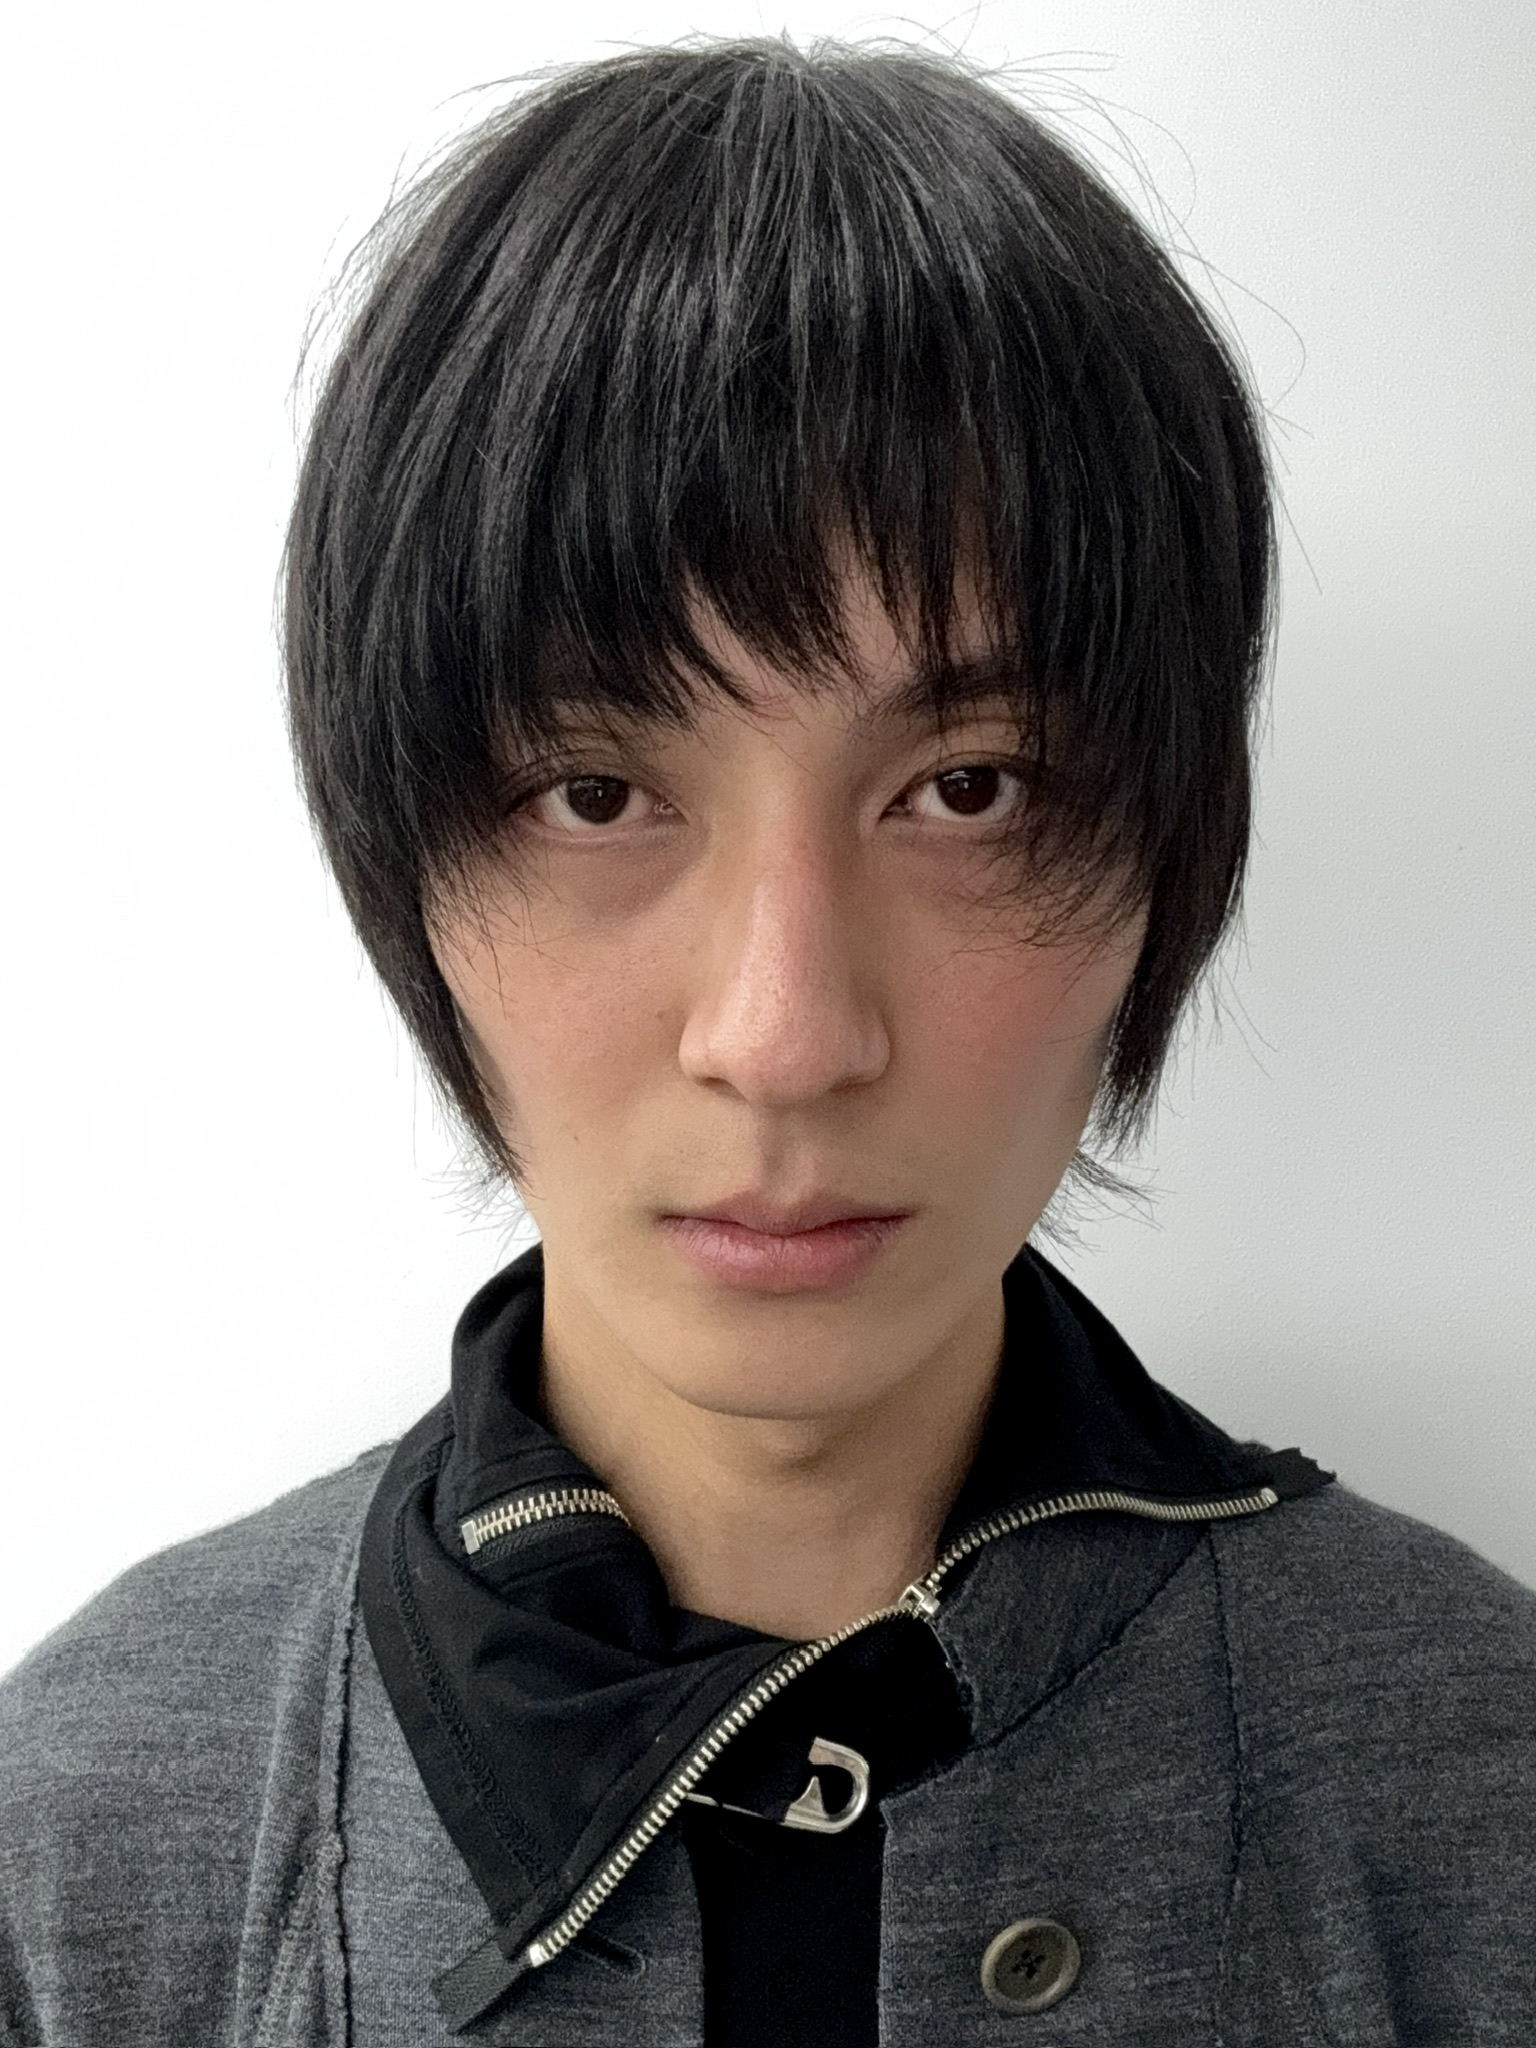
\includegraphics[height=3.5cm]{photo_dlicense.jpeg}
% 	\end{flushleft}
% \end{minipage}
% \hfill
% \begin{minipage}{0.7\textwidth}
% 	\begin{flushright}
% 		{\Huge Edward Hyeonbeen Lee} % Name
% 		\newline\newline
% 		\begin{tabular}{rl}
% 			\textbf{Mobile: }         & \href{tel:+82-10-6236-4693}{+82-10-6236-4693}                                                                 \\
% 			\textbf{EMail: }          & \href{mailto:edward.hyeonbeen.lee@gmail.com}{edward.hyeonbeen.lee@gmail.com}                                  \\
% 			\textbf{GitHub: }         & \href{https://github.com/leehyeonbeen}{github.com/leehyeonbeen}                                               \\
% 			% \textbf{Instagram: } & \href{https://www.instagram.com/leehyeonbeen}{@leehyeonbeen}                                         \\
% 			\textbf{LinkedIn: }       & \href{https://www.linkedin.com/in/hyeonbeen-lee-239500286/}{linkedin.com/in/hyeonbeen-lee-239500286}          \\
% 			\textbf{Google Scholar: } & \href{https://scholar.google.com/citations?user=TiduRxoAAAAJ}{scholar.google.com/citations?user=TiduRxoAAAAJ} \\
% 		\end{tabular}
% 		% \end{center}
% 	\end{flushright}

% \end{minipage}
% % \end{minipage}

% Personal Information Section
% \newcolumntype{L}{>{\raggedright\arraybackslash}m{3.5cm}}
% \newcolumntype{R}{>{\centering\arraybackslash\small}m{4cm}}
% \renewcommand*{\arraystretch}{1.4}
% \noindent
% \section*{PERSONAL INFORMATION}
% \begin{center}
% 	\vspace*{-0.8cm}
% 	\noindent
% 	\begin{longtable}{LRLRLR}
% 		\textbf{Legal Name:}                        & Hyeonbeen Lee                                        & \textbf{Date of birth:} & July 4th, 1996                                   \\
% 		\hline
% 		\textbf{Nationality:}                       & Republic of Korea (South)                            & \textbf{Address:}       & Hoenamu-ro 39gil, Yongsan-gu, Seoul, South Korea \\
% 		\hline
% 		\multirow{3}{*}{\textbf{Military service:}} & \multirow{3}{*}{\shortstack[c]{Honorably discharged,                                                                              \\ Marine Corps Sergeant \\{\small (May 2017$\sim$Feb. 2019)}}} & \multirow{3}{*}{\textbf{Research interest:}} & Robot learning\\ &&& Sensor fusion \\ &&&Sequential decision        \\
% 		\hline
% 	\end{longtable}
% \end{center}


% Education Section
\section*{EDUCATION}
\noindent
\textbf{Virginia Tech}, Blacksburg, VA, USA \hfill Aug. 2026 | May 2031 (Expected)\\ % University name and location
Ph.D. in Mechanical Engineering {\small(Advisor: \href{https://simonstepputtis.com/}{Simon Stepputtis})} \hfill \\ %GPA: -\\
\underline{Research Focus}: Robot Learning, Neurosymbolic AI, Physics-aware ML\\
\\
\textbf{Kyung Hee University}, Seoul, South Korea \hfill Mar. 2022 | Feb. 2024\\ % University name and location
M.Eng. in Mechanical Engineering {\small(Advisor: \href{https://www.jin-gyun-kim.com/}{Jin-Gyun Kim})} \hfill GPA: 3.93/4.0\\ % M.S. 3.933/4.0, 4.10/4.3, 4.33/4.5
\underline{Thesis}: \textsl{{\small `Composite neural network with differential propagation for modeling impulsive nonlinear dynamic systems'}}\\
% \hspace*{1.3cm}\textit{\small{}}\\
% {\small\underline{Coursework}: Probability \& Statistics, Advanced linear algebra, ROS, Computer vision \& Artificial intelligence, Data analysis}\\
\\
\textbf{Kyung Hee University}, Seoul, South Korea \hfill Mar. 2015 | Feb. 2022\\ % University name and location
B.Eng. in Mechanical Engineering {\small(Advisor: \href{https://www.jin-gyun-kim.com/}{Jin-Gyun Kim}, \href{https://scholar.google.com/citations?user=j2drPmMAAAAJ}{Shinkyu Jeong})}\hfill {(\ul{Upper Div.: 3.88/4.0})} GPA: 3.52/4.0\\ % B.S. Overall 3.517/4.0 ,3.599/4.3, 3.84/4.5
% (Upper Div.: 3.878/4.0) (Upper Div.: 4.04/4.3)
% Degree and GPA
\underline{Thesis}: {\small\textsl{{`Data-driven aerodynamic coefficient prediction using deep neural network and PARSEC airfoil parameterization'}}}\\  % B.S. Major 3.509/4.0, 3.573/4.3, ,3.87/4.5 
% \hspace*{1.3cm}\textit{{\small deep neural
% network and PARSEC airfoil parameterization'}} \\
% {\small\underline{Coursework}: Computational dynamics, Robotics, Convex optimization \& Deep learning, Numerical analysis, Finite element methods, Algorithm \& programming, Thermo \& fluid dynamics}\\
% \textbf{Banpo High School}, Science-specialized Track \hfill Mar. 2012 | Feb. 2015
{\footnotesize{($*$ Leave of absence for military service: May 2017 | Feb. 2019)}}

% \noindent
% {Relevant Coursework}:\\
% % \vspace*{0.1cm}\\
% {\renewcommand{\arraystretch}{1.2}
% \begin{tabular}{lll}
% 	$\cdot$ Advanced Linear Algebra (A+) & $\cdot$ Advanced Probability and Statistics (A+) & $\cdot$ Advanced Deep Learning (A-) \\
% 	$\cdot$ Optimization Theory (A+)     & $\cdot$ Numerical Analysis (A+)                  & $\cdot$ System Dynamics (A+)
% \end{tabular}
% }

% \section*{RELEVANT COURSEWORK}
% \vspace*{-0.2cm}
% \begin{tabular}{lll}
% 	$\bullet$ Advanced Linear Algebra (A+) & $\bullet$ Advanced Probability and Statistics (A+) & $\bullet$ Advanced Deep Learning (A-) \\
% 	$\bullet$ Optimization Theory (A+)     & $\bullet$ Numerical Analysis (A+)                  & $\bullet$ System Dynamics (A+)
% \end{tabular}

% \section*{RESEARCH INTERESTS}
% {\small I am currently interested in grounding neurosymbolic policies in physics to enable efficient, interpretable, and generalizable control of robot-environment interactions.}



% Experience Section
\section*{PUBLICATIONS}
\vspace*{-0.2cm}
\subsection*{Journal Papers}
\begin{etaremune}[leftmargin=.5cm, itemsep=0.05cm]
	% \item \textbf{H. Lee}, M. Jung, J.G. Kim et al., “Forecasting high-frequency contact force dynamics via short-time stationarity and freqeuncy-aware neural filters”, \textit{Manuscript in preparation.}
	\item \textbf{H. Lee}, M. Jung, T.K.~Yeu, J.B.~Han, D.~Park, J.G. Kim (2026), ``Frequency-aware decomposition learning for sensorless wrench forecasting on a vibration-rich hydraulic manipulator", submitted to \textit{IEEE/ASME Transactions on Mechatronics.} \href{}{[preprint] \href{https://github.com/leehyeonbeen/FDN}{[code]}}

	\item B. Koo, M. Jung, \textbf{H. Lee}, T. Yeu, J.G. Kim, J.B. Han, Y. Lee, D. Park, “Buoyancy-integrated hybrid reaction force estimation method with real-time haptic feedback for underwater hydraulic manipulation”, submitted to \textit{IEEE Robotics and Automation Letters.} % {\small({$*$ Formal authorship addition is currently in process})}

	\item \textbf{H. Lee}, S. Han, H.S. Choi, J.G. Kim (2024), “cNN-DP: Composite neural network with differential propagation for impulsive nonlinear dynamics”, \textit{Journal of Computational Physics (WoS IF Top 2.5\% in Physics, Mathematical)}, 496, 112578. \href{https://www.sciencedirect.com/science/article/pii/S0021999123006733}{[link]} \href{https://github.com/leehyeonbeen/cNN-DP}{[code]}

	\item S. Han$^*$, G.E. Jeong$^*$, \textbf{H. Lee}, W.S. Choi, J.G. Kim (2023), “Multi-body dynamics model for spent nuclear fuel transportation system under normal transport test conditions”, \textit{Nuclear Engineering and Technology (WoS IF Top 13.7\% in Nuclear Science \& Technology)}, 55(11), 4125-4133. {\small ($^*$Co-first authors)} \href{https://www.sciencedirect.com/science/article/pii/S1738573323003492}{[link]}
\end{etaremune}

\vspace*{-0.6cm}
\subsection*{Conferences \& Proceedings}
\begin{etaremune}[leftmargin=.5cm, itemsep=0.05cm]
	\item J.H. Han, J.B. Han, S.S. Kim, M.H. Kim, Y.H. Kim, \textbf{H. Lee}, J.G. Kim, T.K. Yeu. “Digital twin model of underwater construction robot for real-time grinding simulation”, \textit{7th International Conference on Multibody System Dynamics}, Madison, WI, USA, Jun. 2024 \href{https://easychair.org/publications/preprint/WkF3}{[link]}
	\item \textbf{H. Lee}, J. Han, T.K. Yeu, J.G. Kim. “Real-time multi-horizon reaction force forecasting of marine robot using interpretable Transformer”, \textit{Korean Society of Mechanical Engineers} (Oral Presentation), Incheon, South Korea, Nov. 2023  \href{https://www.dbpia.co.kr/Journal/articleDetail?nodeId=NODE11709087}{[link]}
	\item \textbf{H. Lee,} S. Han, H.S. Choi, J.G. Kim. “Meta-modeling of nonlinear impulsive dynamics using composite neural network model with differential propagation”, \textit{Korean Society of Mechanical Engineers} (\textbf{Excellent Paper Award}, Oral Presentation, $*$ Extended works from IMAC 2023), Busan, South Korea, May 2023. \href{https://www.dbpia.co.kr/journal/articleDetail?nodeId=NODE11511050}{[link]}
	% \item \textbf{H. Lee,} S. Han, H.S. Choi, J.G. Kim. “Composite neural network with differentiation propagation for modeling nonlinear impulsive dynamics”, \textit{Conference on Dynamics and Control, Korean Society of Mechanical Engineers} (Oral Presentation), Jeju, South Korea, Mar 2023 \href{https://www.dbpia.co.kr/Journal/articleDetail?nodeId=NODE11527668}{[link]}
	\item \textbf{H. Lee,} S. Han, H.S. Choi, J.G. Kim. “Composite neural network framework for modeling impulsive nonlinear dynamic responses”, \textit{41st International Modal Analysis Conference (IMAC)} (Oral Presentation), Austin, TX, USA, Feb. 2023 \href{https://link.springer.com/chapter/10.1007/978-3-031-34946-1_21}{[link]}
	\item \textbf{H. Lee}, J.G. Kim. “Development of multibody dynamics trailer model using normal transportation test data and DNN based surrogate model generation”, \textit{Korean Society for Noise and Vibration Engineering} (Oral Presentation), Jeju, South Korea, Dec 2022
\end{etaremune}

\section*{AWARDS \& HONORS}
\begin{itemize}
	\item \textbf{Excellent Paper Award} \hfill Korean Society of Mechanical Engineers, 2023 % No.2023-083, Aug 25 2023
		      {\small
			      \vspace*{-0.2cm}
			      \begin{itemize}
				      \item Awarded for a first-author presentation on physics-aware modeling of nonlinear dynamics.
			      \end{itemize}}
	      \vspace*{-0.2cm}
	\item \textbf{Brain Korea 21 Plus Scholarship}\hfill Graduate School, Kyung Hee University, 2022 | 2023 % KRW 23,340,000
	{\small
			      \vspace*{-0.2cm}
			      \begin{itemize}
				      \item Received \$16K in graduate funding during M.Eng. studies.
			      \end{itemize}}
	      \vspace*{-0.2cm}
	\item \textbf{Graduate Assistantship} \hfill Graduate School, Kyung Hee University, 2022 | 2023 % KRW 16,046,400
		      {\small
			      \vspace*{-0.2cm}
			      \begin{itemize}
				    %   \item Appointed as lead departmental assistant and received additional funding for master's studies.
					\item Received \$11K through a selective graduate assistantship during M.Eng. studies.
			      \end{itemize}}
	      \vspace*{-0.2cm}
	\item \textbf{Academic Superiority Scholarship} \hfill Dept. of Mechanical Engineering, Kyung Hee University, Spring 2021 % Mar. % KRW 4,290,000
		      {\small
			      \vspace*{-0.2cm}
			      \begin{itemize}
					\item \ul{Ranked 1st} in the GPA-based departmental merit review and received a full tuition waiver valued at \$3K.
				    %   \item \ul{Ranked 1st} among departmental scholarship candidates and received a full tuition waiver. % 4th year 7/200, 185 graduating, 1/15
			      \end{itemize}}
\end{itemize}


\newgeometry{left=1cm, right=1cm, top=1.5cm, bottom=1.5cm}
\section*{RESEARCH EXPERIENCES}
% \setitemize{itemsep=0cm}
\noindent\textbf{Graduate School, Kyung Hee University} \hfill Postgraduate Researcher\\
Modeling \& Simulation Lab., advised by \textsl{Jin-Gyun Kim} \hfill Mar. 2024 | Apr. 2026\\
\vspace*{-0.25cm}\\
\begin{minipage}{0.78\textwidth}
	\footnotesize
	\begin{itemize}
		\item Accelerated and improved the force model for real-time deployment in the control loop for \href{https://www.kriso.re.kr/eng/}{\underline{KRISO}}. Independently secured the project for a year.
		\item Combined decomposition-based probabilistic modeling, frequency-aware architectures, and proprioception-to-wrench transfer learning to sensorlessly forecast contact- and vibration-rich wrench of a robotic manipulator. Submitted a first-authored manuscript to the \textit{IEEE/ASME Transactions on Mechatronics (T-MECH)}.
		      % \item Executed a national research grant (\href{https://www.kriso.re.kr/eng/}{KRISO}) by improving the accuracy and inference speed of the force forecasting model.
		      % \item Accelerated inference by structural parallelization, compiling, and mixed precision for real-time system application.
	\end{itemize}
\end{minipage}\\

% \noindent\textbf{Freelance AI Researcher} \hfill \\
% \null \hfill Mar. 2024 | Present\\
% \vspace*{-0.25cm}\\
% \begin{minipage}{0.77\textwidth}
%   \small
%   \begin{itemize}
%       \item Developed a scalable framework for forecasting high-frequency forces of robot in contact-rich manipulation scenarios.
%             % \item Accelerated inference by structural parallelization, compiling, and mixed precision for real-time system application.
%   \end{itemize}
% \end{minipage}\\

% \noindent\textbf{Freelance AI developer} \hfill Freelancer\\
% --- \hfill Mar. 2024 | Present\\
% \hspace*{0.46cm}

% \vspace*{0.12cm}
\noindent\textbf{Kim Jaechul Graduate School of AI, KAIST} \hfill Research Engagement\\
Cognitive Learning for Vision \& Robotics Lab., advised by \textsl{Joseph J. Lim} \hfill Sep. 2023 | Nov. 2023\\
\vspace*{-0.25cm}\\
\begin{minipage}{0.77\textwidth}
	\footnotesize
	\begin{itemize}
		\item Conducted a literature review on \href{https://clvrai.github.io/spirl/}{\ul{skill prior regularized reinforcement learning (SPiRL)}} and delivered a 90-minute technical presentation to lab members and faculty.
		% \item Received a formal internship offer from the lab director following the presentation (offer later declined).
		      % \item Analyzed skill prior accelerated reinforcement learning (SPiRL), and delivered a technical presentation to the lab.
		      % \item Investigated reinforcement learning for robots and skill prior extraction methodologies for learning-based long-horizon robot control.
	\end{itemize}
\end{minipage}\\


\noindent\textbf{Graduate School, Kyung Hee University} \hfill Master's Student\\
Modeling \& Simulation Lab., advised by \textsl{Jin-Gyun Kim} \hfill Mar. 2022 | Feb. 2024\\
\vspace*{-0.25cm}\\
\begin{minipage}{0.77\textwidth}
	\footnotesize
	\begin{itemize}
		\item Proposed a novel neural network architecture for learning complex dynamics from multi-order derivatives. Published a first-author article in the \textit{Journal of Computational Physics (JCOMP)}.
		\item Developed a neural metamodel of real-world vehicle dynamics with high-fidelity physics simulation for the \href{https://www.kaeri.re.kr/eng/}{\ul{Korea Atomic Energy Research Institute (KAERI)}}. Published a co-authored article in the \textit{Nuclear Engineering and Technology (NET)}.
		\item Designed a probabilistic frequency-aware model to forecast contact-rich wrench of a hydraulic manipulator for the \href{https://www.kriso.re.kr/eng/}{\ul{Korea Research Institute of Ships and Ocean Engineering (KRISO)}}. Independently and successfully secured the project for two years.
		% \item Actively explored and implemented methods from diverse ML domains including time-series forecasting, computer vision, physics-informed learning, and system identification.
		      % \item Implemented foundational deep models from scratch, adapting them to analyze multi-modal [force/vision] data from real-world
	\end{itemize}
\end{minipage}\\

\vspace*{0.1cm}
\noindent\textbf{Department of Mechanical Engineering, Kyung Hee University} \hfill Undergraduate Researcher\\
Modeling \& Simulation Lab., advised by \textsl{Jin-Gyun Kim} \hfill Jan. 2021 | Feb. 2022\\
\vspace*{-0.25cm}\\
\begin{minipage}{0.77\textwidth}
	\footnotesize
	\begin{itemize}
		\item Investigated data-driven methods for flexible multibody dynamics as part of a government-funded research project on vehicle dynamics simulation.
	\end{itemize}
\end{minipage}\\
\vspace*{-0.2cm}





% \textbf{Pre-Ph.D Research Intern} \hfill Sep. 2023 | Dec. 2023\\
% Cognitive Learning for Vision \& Robotics Lab., Graduate School of AI, KAIST \hfill \\
% --- \textsl{Skill-based reinforcement learning, Skill prior extraction}\\
% \textbf{Undergraduate Research Intern} \hfill Jan. 2021 | Feb. 2022\\
% Modeling \& Simulation Lab., Dept. of Mechanical Eng., Kyung Hee University\\
% --- \textsl{Data-driven flexible multi-body dynamics, Composite neural network}

% \section*{CAREER}
% \noindent
% \textbf{8DIVISION}, Flagship Store Staff \hfill Feb. 2024 | Present
% \begin{itemize}
% 	\item Global fashion sales
% 	\item \textbf{Creative social media management (@8division, @8division$\_$journal)}
% 	\item Modeling and styling
% 	\item Robotic process automation using Python Selenium
% 	\item Sales analysis using Python dataprocessing libs
% \end{itemize}
% \textbf{Freelance model}\hfill May 2024 | Present
% \begin{itemize}
% 	\item \href{https://instagram.com/gyoureekim}{@gyoureekim} SS2025 fitting model for \href{https://instagram.com/londonfashionweek}{London Fashion Week}
% 	\item \href{https://instagram.com/san263_1}{@san263$\_$1} FW2024/SS2025 fitting model
% 	\item \href{https://instagram.com/8division}{@8division}, \href{https://instagram.com/8division_journal}{@8division$\_$journal} store fitting model
% 	\item \href{https://instagram.com/armed_dept}{@armed$\_$dept} FW2024 Lookbook
% 	\item Personal works with photographers: \href{https://instagram.com/chtewon}{@chtewon}, \href{https://instagram.com/wyw_kiki98}{@wyw$\_$kiki98}, \href{https://instagram.com/leeejaehoon}{@leeejaehoon}, \href{https://instagram.com/jngsnghun}{@jngsnghun}
% 	\item Magazines: \href{https://instagram.com/pap_magazine}{@pap$\_$magazine}, \href{https://instagram.com/prism.mag}{@prism.mag}
% \end{itemize}

% \section*{LANGUAGE}
% \subsection*{}
% \begin{itemize}
% 	\item English
% 	      \begin{itemize}
% 		      \item \textbf{Certification - New TEPS 513/600} (equivalent to 980/990 in ETS TOEIC)
% 		      \item \textbf{Certification - ACTFL OPI English AH(Advanced High)}
% 		      \item Expertised communication ability in native level
% 		      \item Rich communication experiences with global fashion creatives and designers
% 		      \item Published two papers for international science journals as first and co-author
% 		      \item Abundant experiences at international conference presentations, research meetings, and email communication in expert levels
% 	      \end{itemize}
% 	\item Japanese
% 	      \begin{itemize}
% 		      \item Able to speak daily-level conversations
% 		      \item Understands movies and TV shows in Japanese without subtitles
% 	      \end{itemize}
% \end{itemize}

% \subsection*{Global networking}
% Possesses communications, collaborations and socialization experiences with non-Korean fashion brands or influencers listed below:\\\\
% \noindent
% {\textbf{English speakers}}
% \begin{tasks}[style=itemize](3)
% 	\task Stefan Cooke \& Jake Burt
% 	\task SABUKARU
% 	\task Betsy Johnson
% 	\task RIER
% 	\task ThinkingMU
% 	\task FFFPostalService
% 	\task Luca Hamers
% 	\task GR10K
% 	\task Untitled Agency
% 	\task Bonnie \& Clyde
% 	\task SAMUTARO
% 	\task Hiking Patrol
% 	\task \_J.L-A.L\_
% 	\task Stockholm Surfboard Club
% 	\task JUS Stockholm
% 	\task DOUBLEU
% \end{tasks}

% \noindent
% {\textbf{Japanese speakers}}
% \begin{tasks}[style=itemize](3)
% 	\task Nepenthes
% 	\task KAMIYA
% 	\task PickYou
% 	\task COMOLI
% 	\task Ken Mitsuishi
% 	\task NorthWorks
% 	\task Huntism Tokyo
% 	\task OURs (YouTube)
% 	\task JunctionJP
% 	\task HLTVC
% \end{tasks}

% Experience Section
% \section*{CONFERENCES}
% \begin{etaremune}[leftmargin=.5cm, itemsep=0.05cm]
% \noindent
% \newcolumntype{L}{>{\raggedright\arraybackslash}m{14cm}}
% \newcolumntype{R}{>{\raggedright\arraybackslash}m{5cm}}
% \vspace*{-.5cm}
% \begin{longtable}{LR}
% 	J.H. Han, J.B. Han, S.S. Kim, M.H. Kim, Y.H. Kim, \textbf{H. Lee}, J.G. Kim, T.K. Yeu. “Digital twin model of underwater construction robot for real-time grinding simulation”, \textit{7th International Conference on Multibody System Dynamics.} \href{https://easychair.org/publications/preprint/WkF3}{[link]}                                                                                              & {Jun. 9 2024 \linebreak Madison, WI, USA}     \\
% 	\textbf{H. Lee}, J. Han, T.K. Yeu, J.G. Kim. “Real-time multi-horizon reaction force forecasting of marine robot using interpretable Transformer”, \textit{Korean Society of Mechanical Engineers} (Oral Presentation). \href{https://www.dbpia.co.kr/Journal/articleDetail?nodeId=NODE11709087}{[link]}                                                                                                         & {Nov. 1 2023 \linebreak Incheon, South Korea} \\
% 	\textbf{H. Lee,} S. Han, H.S. Choi, J.G. Kim. “Meta-modeling of nonlinear impulsive dynamics using composite neural network model with differential propagation”, \textit{Korean Society of Mechanical Engineers} (\textbf{Excellent Paper Award}, Oral Presentation). {\small($*$ Extended works from IMAC 2023 presentation)} \href{https://www.dbpia.co.kr/journal/articleDetail?nodeId=NODE11511050}{[link]} & {May 18 2023 \linebreak Busan, South Korea}   \\
% 	% \href{https://www.dbpia.co.kr/Journal/articleDetail?nodeId=NODE11527668}{\textbf{H. Lee,} S. Han, H.S. Choi, J.G. Kim. “Composite Neural Network with Differentiation Propagation for Modeling Nonlinear Impulsive Dynamics”, \textit{Conference on Dynamics and Control, Korean Society of Mechanical Engineers} (Oral Presentation)}.                                        & {Mar. 23 2023 \linebreak Jeju, South Korea}   \\
% 	\textbf{H. Lee,} S. Han, H.S. Choi, J.G. Kim. “Composite neural network framework for modeling impulsive nonlinear dynamic responses”, \textit{41st International Modal Analysis Conference (IMAC)} (Oral Presentation). \href{https://link.springer.com/chapter/10.1007/978-3-031-34946-1_21}{[link]}                                                                                                           & {Feb. 16 2023 \linebreak  Austin, TX, USA}    \\
% 	\textbf{H. Lee}, J.G. Kim. “Development of multibody dynamics trailer model using normal transportation test data and DNN based surrogate model generation”, \textit{Korean Society for Noise and Vibration Engineering} (Oral Presentation).                                                                                                                                                                    & {Dec. 4 2022 \linebreak Jeju, South Korea}    \\
% \end{longtable}

\section*{SKILLS}
\begin{itemize}
	\item \textbf{Programming Languages: }Python $\cdot$ MATLAB $\cdot$ C++ $\cdot$ \LaTeX
	\item \textbf{Software \& Frameworks: }PyTorch $\cdot$ Git $\cdot$ Docker $\cdot$ ROS $\cdot$ RecurDyn $\cdot$ Gazebo $\cdot$ MuJoCo $\cdot$ OpenAI API
	      % \item \textbf{Machine Learning: }Time series forecasting $\cdot$ Skill-based reinforcement learning $\cdot$ Image segmentation $\cdot$ Self-supervised learning $\cdot$ $\cdot$ Physics-informed learning $\cdot$ Frequency domain learning $\cdot$ Foundation model fine-tuning
	\item \textbf{Scientific Computing: }Flexible multibody dynamics $\cdot$ Finite element methods $\cdot$ Numerical analysis
	\item \textbf{Natural Languages: }Korean (Native) $\cdot$ English (TOEFL iBT 111/120) $\cdot$ Japanese (Advanced proficiency)
	      %   \begin{itemize}
	      %       \item \textit{Expertised at handling \underline{sequential data and models}}
	      %   \end{itemize}
	      % \item \textbf{English: }Speaks at native level
	      % \item \textbf{Japanese: }Speaks at intermediate level
\end{itemize}


\section*{INVITED SEMINARS}
\begin{etaremune}[leftmargin=.5cm, itemsep=0.05cm]
\item ``\textsl{On the data-driven modeling of contact- and vibration-rich dynamics}", invited seminar, IMBD Lab, Chungnam National University, Daejeon, South Korea, Apr. 16, 2026 \href{https://drive.google.com/file/d/1NrgUaUlQ5dAOx_Jav5x5ZCGPavyc7Ayj/view?usp=sharing}{[keynote]}
\item ``\textsl{On the data-driven modeling of contact- and vibration-rich dynamics}", invited seminar, Modeling \& Simulation Lab, Kyung Hee University, Yongin, South Korea, Apr. 14, 2026 \href{https://drive.google.com/file/d/1NrgUaUlQ5dAOx_Jav5x5ZCGPavyc7Ayj/view?usp=sharing}{[keynote]}
\end{etaremune}



% Experience Section
\setlength{\itemsep}{10pt} % Set to 0 to remove space
\section*{SELECTED PROJECTS}
\begin{itemize}
	\item Segment-Anybody, at \textit{Dept. of AI, Kyung Hee University} \href{https://github.com/leehyeonbeen/segment-anything-fine-tuning}{[code]}

	      {\footnotesize
		      \vspace*{-0.2cm}
		      \begin{itemize}
			      \item Fine-tuned Meta's Segment-Anything Model (SAM) for detailed human body parts segmentation in human-robot interaction.
		      \end{itemize}
		      \vspace*{-0.2cm}
	      }

	\item Deep seq2seq from scratch, \textit{Personal project}. \href{https://github.com/leehyeonbeen/TimeSeriesSeq2Seq}{[code]}

	      {\footnotesize
		      \vspace*{-0.2cm}
		      \begin{itemize}
			      \item Scratch-implemented deep sequence-to-sequence models, from RNN to Transformer variants.
		      \end{itemize}
		      \vspace*{-0.2cm}
	      }

	\item ROS SLAM on Apple Silicon devices, \textit{Personal project}. \href{https://github.com/leehyeonbeen/ROS-SLAM-AppleSilicon}{[code]}

	      {\footnotesize
		      \vspace*{-0.2cm}
		      \begin{itemize}
			      \item Addressed ROS TurtleBot3 SLAM and Gazebo compatibility issues on the Apple Silicon MacOS devices.
		      \end{itemize}
		      \vspace*{-0.2cm}
	      }



	% \item cNN-DP, at \textit{Modeling \& Simulation Lab}. \href{https://github.com/leehyeonbeen/cNN-DP}{[code]}

	%       {\footnotesize
	% 	      \vspace*{-0.2cm}
	% 	      \begin{itemize}
	% 		      \item Official implementation of the \textit{Journal of Computational Physics} paper.
	% 	      \end{itemize}
	% 	      \vspace*{-0.2cm}
	%       }

	\item RecurDyn ProcessNet with Python, at \textit{Modeling \& Simulation Lab}. \href{https://github.com/leehyeonbeen/RecurDynPython}{[code]}

	      {\footnotesize
		      \vspace*{-0.2cm}
		      \begin{itemize}
			      \item Automated and parallelized flexible multibody dynamics (FMBD) simulations of RecurDyn.
		      \end{itemize}
		      \vspace*{-0.2cm}
	      }
\end{itemize}
% \noindent
% \newcolumntype{L}{>{\raggedright\arraybackslash}m{13cm}}
% \newcolumntype{R}{>{\raggedright\arraybackslash}m{4cm}}
% \vspace*{-.6cm}
% \begin{longtable}{LR}
% 	% \underline{Ongoing:} Probabilistic-Deterministic Hybrid Fourier Networks for High-Frequency Sensor Dynamics
% 	% Deep-learning based reaction force and torque prediction model development for underwater ground cutting robot using experimental measurements and dynamic simulation data, Korea Research Institute of Ships and Ocean Engineering (KRISO). (\textit{Manuscript in preparation}) & {Mar. 2022 | Present}   \\

% 	% {Apr. 2024 | May. 2024} & Automatic products registration, 8DIVISION. (\href{github.com/leehyeonbeen/AfterCompany-AutoProductReg}{github.com/leehyeonbeen/AfterCompany-AutoProductReg})                                                                                                              \\

% 	$\bullet$ cNN-DP: Composite neural network with differential propagation for impulsive nonlinear dynamics, Modeling \& Simulation Lab. (\href{https://github.com/leehyeonbeen/cNN-DP}{github.com/leehyeonbeen/cNN-DP})                                                              & {Nov. 2021 | Jan. 2024} \\

% 	% Metamodel generation and evolution procedures for flexible multibody dynamics, FunctionBay Inc.                                                                                                                                                                            & {Sep. 2021 | Jan. 2024} \\

% 	$\bullet$ ROS SLAM setup package distribution for Apple Silicon devices, Personal project. (\href{https://github.com/leehyeonbeen/ROS-SLAM-AppleSilicon}{github.com/leehyeonbeen/ROS-SLAM-AppleSilicon})                                                                            & {Sep. 2023 | Oct. 2023} \\

% 	$\bullet$ Bottom-Up codes development of time series AI models: From RNN to advanced Transformers, Personal project. (\href{https://github.com/leehyeonbeen/TimeSeriesSeq2Seq}{github.com/leehyeonbeen/TimeSeriesSeq2Seq})                                                          & {Mar. 2022 | Aug. 2023} \\

% 	$\bullet$ Segment Anyone: Fine-tuned Segment-Anything-Model (SAM) for human-collaborative robots, Kyung Hee University Dept. of Artifical Intelligence. (\href{https://github.com/leehyeonbeen/segment-anything-fine-tuning}{github.com/leehyeonbeen/segment-anything-fine-tuning}) & {Mar. 2023 | Jun. 2023} \\

% 	$\bullet$ RecurDyn Automation using Python, Modeling \& Simulation Lab. (\href{https://github.com/leehyeonbeen/RecurDynPython}{github.com/leehyeonbeen/RecurDynPython})                                                                                                             & {Dec. 2022 | Jun. 2023} \\

% 	% Development of ground·sea transportation test simulation model using multibody dynamics and DNN-based metamodel, Korea Atomic Energy Research Institute (KAERI). (Codes under classification.)                                                                             & {Sep. 2021 | Oct. 2022} \\
% \end{longtable}

% % % Experience Section
% \section*{GRANTS}
% \noindent
% \newcolumntype{L}{>{\raggedright\arraybackslash}m{13cm}}
% \newcolumntype{R}{>{\raggedright\arraybackslash}m{4cm}}
% \vspace*{-.5cm}
% \begin{longtable}{LR}
% 	Deep-learning based reaction force prediction of underwater excavation robot using experimental measurements and dynamic simulation, \href{https://www.kriso.re.kr/eng/}{\textit{Korea Research Institute of Ships and Ocean Engineering (KRISO)}.} & {Mar. 2022 | Oct. 2024} \\

% 	Metamodel generation and evolution procedures for flexible multibody dynamics, \href{https://functionbay.com/en}{\textit{FunctionBay Inc.}}                                                                                                         & {Mar. 2021 | Feb. 2024} \\
% 	% {Apr. 2024 | May. 2024} & Automatic products registration, 8DIVISION. (\href{github.com/leehyeonbeen/AfterCompany-AutoProductReg}{github.com/leehyeonbeen/AfterCompany-AutoProductReg})                                                                                                              \\

% 	% 	% {Nov. 2021 | Jan. 2024} & cNN-DP: Composite neural network with differential propagation for impulsive nonlinear dynamics, Modeling \& Simulation Lab. (\href{https://github.com/leehyeonbeen/cNN-DP}{github.com/leehyeonbeen/cNN-DP})                                                               \\
% 	% 	Metamodel generation and evolution procedures for flexible multibody dynamics, \textit{FunctionBay Inc.}                                                                                                       & {Sep. 2021 | Jan. 2024} \\

% 	% 	% {Sep. 2023 | Oct. 2023} & ROS SLAM setup package distribution for Apple Silicon devices, Personal project. (\href{github.com/leehyeonbeen/ROS-SLAM-AppleSilicon}{github.com/leehyeonbeen/ROS-SLAM-AppleSilicon})                                                                                     \\

% 	% 	% {Mar. 2022 | Aug. 2023} & Bottom-Up codes development of time series AI models: From RNN to advanced Transformers. (\href{github.com/leehyeonbeen/TimeSeriesSeq2Seq}{github.com/leehyeonbeen/TimeSeriesSeq2Seq})                                                                                     \\

% 	% 	% {Mar. 2023 | Jun. 2023} & Segment Anyone: Fine-tuned Segment-Anything-Model (SAM) for human-collaborative robots, Kyung Hee University Dept. of Artifical Intelligence. (\href{https://github.com/leehyeonbeen/segment-anything-fine-tuning}{github.com/leehyeonbeen/segment-anything-fine-tuning})  \\
% 	% 	% {Dec. 2022 | Jun. 2023} & RecurDyn Automation using Python, Modeling \& Simulation Lab. (\href{https://github.com/leehyeonbeen/RecurDynPython}{github.com/leehyeonbeen/RecurDynPython})                                                                                                              \\
% 	Development of ground·sea transportation test simulation model using multi-body dynamics and DNN-based metamodel, \href{https://www.kaeri.re.kr/eng/}{\textit{Korea Atomic Energy Research Institute (KAERI).}}                                     & {Sep. 2021 | Oct. 2022} \\
% \end{longtable}

\section*{TEACHING \& MENTORSHIP}
\textbf{Research Mentor} \hfill Modeling \& Simulation Lab., Kyung Hee University\\
--- {\footnotesize{Guiding junior graduate students on robotics and machine learning.}} \hfill Mar. 2025 | Present\\ % Mar. 2022 | Jun. 2023
\vspace*{-0.2cm}

\noindent
\textbf{Teaching Assistant, ME380 Systems Dynamics} \hfill Dept. of Mechanical Engineering, Kyung Hee University\\
--- {\footnotesize{Lectured on multibody dynamics with theoretical derivation and its computational implementation.}} \hfill Mar. 2022 | Jun. 2023 % Mar. 2022 | Jun. 2023

% Skills Section
% \section*{CERTIFICATES}
% \begin{itemize}
% 	\item \textbf{New TEPS:} 513/600 (equivalent to TOEIC 980/990) \hfill No.0111736, Valid, May 13 2023

% 	\item \textbf{ACTFL OPI English:} AH (Advanced High) \hfill 2A7617334333, Valid, Nov. 14 2023
% 	      % \item \textbf{RA Scholarship (80\% tuition)} \hfill Kyung Hee University, Sep. 01 2023
% 	      % \item \textbf{Exellence Paper Award} \hfill Korean Society of Mechanical Engineers, No.2023-083, Aug. 25 2023
% 	      % \item \textbf{RA Scholarship (80\% tuition)} \hfill Kyung Hee University, Mar. 01 2023
% 	      % \item \textbf{RA Scholarship (80\% tuition)} \hfill Kyung Hee University, Sep. 01 2022
% 	      % \item \textbf{행정조교 장학금} \hfill 경희대학교 대학원, 수혜년월: 2022.09 | 2024.02
% 	      % \item \textbf{Excellence Scholarship (Full tuition)} \hfill Kyung Hee University, Mar. 01 2021
% 	\item \textbf{TOEIC:} 925/990 \hfill No.605083, Expired, Nov. 25 2018
% \end{itemize}



% \textbf{Representative Administration Assistant} \hfill Dept. of Mechanical Eng., Kyung Hee University, Sep 2022 | Present\\
% \textbf{Multibody dynamics} \hfill Kyung Hee University, Mar 2022 | Jun 2023\\
% \noindent
% \newcolumntype{L}{>{\raggedright\arraybackslash}m{12cm}}
% \newcolumntype{R}{>{\raggedright\arraybackslash}m{5cm}}
% \vspace*{-.5cm}
% \begin{longtable}{LR}
% 	\textbf{Administration Assistant} & Dept. of Mechanical Eng., Kyung Hee University
% \end{longtable}
% Experience Section
% \section*{사회경험}
% \noindent
% \textbf{맥도날드 서울교대점} 고객응대, 주방보조, 계산 \hfill 2014.11 - 2015.02\\
% \textbf{육회한연어 수원영통점} 서빙, 주방보조, 계산 \hfill 2016.02 - 2016.06\\
% \textbf{슈펜 가로수길점} 외국인 고객응대, 물류창고정리 \hfill 2016.06 - 2016.09\\
% \textbf{오늘 와인한잔 수원역점} 서빙, 주방보조 \hfill 2016.09 - 2016.12\\
% \textbf{아이리스 BAR} 서빙, 주방보조, 고객응대 \hfill 2019.03 - 2019.06\\
% \textbf{대명GEC} 삼성전자 화성사업장 케이블 배선작업 \hfill 2019.07 - 2019.08\\
% \textbf{Seminar: IAS18 Workshop\&Tutorials} \hfill {\small Intl. Conference on Intelligent Autonomous Systems}, Jul 2023\\
% \textbf{Seminar: AI Summer School 2022} \hfill Korean Society of Mechanical Engineers, Aug 2022\\
% \textbf{Teaching Assistant (System Dynamics)} \hfill Modeling \& Simulation Lab, Mar 2022 - Jun 2023\\
% \textbf{Seminar: AI Summer School 2021} \hfill Korean Society of Mechanical Engineers, Aug 2021\\
% \textbf{Seminar: AI, Data Driven Models\&ML} \hfill {\small National Agency Finite Element Methods and Standard}, Apr 2021\\
% \textbf{Undergraduate Research Internship} \hfill Modeling \& Simulation Lab, Jan 2021 | Feb 2022\\
% \textbf{48th Student Council} \hfill Kyung Hee University College of Engineering, Feb 2019 | Jan 2020\\
% \textbf{R.O.K.-U.S. Combined Marine Corps Interpreter} \hfill 1st Marine Div., ROKMC, Sep 2017 | Feb 2019\\



% \section*{SEMINARS}
% \textbf{Intl. Conference on Intelligent Autonomous Systems} \hfill Workshops \& Tutorials, Jul. 2023\\
% \textbf{Korean Society of Mechanical Engineers} \hfill AI Summer Camp, Aug. 2022\\
% \textbf{Korean Society of Mechanical Engineers} \hfill AI Summer Camp, Aug. 2021\\
% \textbf{\small National Agency for Finite Element Methods and Standards} \hfill {Seminar on data-driven models}, Apr. 2021\\


% Experience Section
\section*{COMMUNITY SERVICE}
% \textbf{Representative Administrative Assistant} \hfill Kyung Hee University, Sep 2022 | Present\\
% \textbf{Seminar: IAS18 Workshop \& Tutorials} \hfill {\small Intl. Conference on Intelligent Autonomous Systems}, Jul. 2023\\
% \textbf{Seminar: AI Summer School 2022} \hfill Korean Society of Mechanical Engineers, Aug. 2022\\
% \textbf{Teaching Assistant (System Dynamics)} \hfill Modeling \& Simulation Lab, Mar 2022 - Jun 2023\\
% \textbf{Seminar: AI Summer School 2021} \hfill Korean Society of Mechanical Engineers, Aug. 2021\\
% \textbf{Seminar: AI, Data Driven Models \& ML} \hfill {\small National Agency Finite Element Methods and Standard}, Apr. 2021\\
% \textbf{Fashion Model} \hfill East Casting Agency, Mar. 2024 | Present\\
\textbf{Lead Administrative Assistant} \hfill Dept. of Mechanical Engineering, Kyung Hee University, 2022 | 2024\\
% \null\hfill \\ % Sep. 2022 | Feb. 2024
\textbf{College of Engineering 48th Student Council} \hfill Kyung Hee University, Feb 2019 | Jan. 2020\\
% \null\hfill \\
\textbf{R.O.K.-U.S. Combined Marine Corps Interpreter} \hfill 1st Marine Div., ROKMC, Sep 2017 | Feb. 2019
% End document

\section*{REFERENCES}
\begin{itemize}
	\item \textbf{Jin-Gyun Kim}, Ph.D.

	      \quad {\small Associate Professor at Department of Mechanical Engineering, Kyung Hee University (\href{mailto:jingyun.kim@khu.ac.kr}{jingyun.kim@khu.ac.kr})}


	\item \textbf{Hee-Sun Choi}, Ph.D.

	      \quad{\small Assistant Professor at Department of Artificial Intelligence and Robotics, Sejong University (\href{mailto:heesunchoi@sejong.ac.kr}{heesunchoi@sejong.ac.kr})}%{\Vhrulefill} 

	\item \textbf{Seongji Han}, Ph.D.

	      \quad{\small Assistant Professor at Department of Mechatronics Engineering, Chungnam National University (\href{mailto:seongji.han@cnu.ac.kr}{seongji.han@cnu.ac.kr})}
\end{itemize}


\end{document}
